

%%%%%%%%%%%%%%%%%%%%%%%%%%%%%%%%%%%55%%
\begin{frame} [plain]
    \frametitle{}
    \Background[1] 
    \begin{center}
    {\huge 第5讲:量子算法(1)    }
    \end{center}  
    \addtocounter{framenumber}{-1}   
\end{frame}
%%%%%%%%%%%%%%%%%%%%%%%%%%%%%%%%%%

\section{1.量子算法的特点}
\begin{frame}
    \frametitle{量子并行性}
    \begin{itemize}
        \Item 量子算法的根本特点是量子并行性
        \Item 与经典并行性的根本区别:\\
        \begin{itemize}
            \IItem 经典计算每条线路计算一个分支任务,多条线路共同完成并行任务 \\
            量子计算一条线路完成所有分支的计算任务
            \IItem 经典计算各分支计算所需时间不同时,大量线路出现等待情况。 \\
            量子并行各分支同时完成计算
        \end{itemize}
    \end{itemize}
\end{frame}

\begin{frame} 
        \frametitle{}
    杨子见歧道而哭之
    \begin{center}
        
\includegraphics[width=0.5\textwidth]{figs/33.png}
    \end{center}
\end{frame}

\section{2. 多伊奇算法}
\begin{frame}
    \frametitle{Deutsch 算法}
    {\Bullet}~分析:二进制函数$f(x)$的特点
    \begin{table} 
    \begin{tabular}{ccccc}
        \toprule
         & $f_1(x)$ & $f_2(x)$ & $f_3(x)$ & $f_4(x)$ \\
        \midrule
        x=0 & 0 & 0 & 1 & 1\\
        x=1 & 0 & 1 & 0 & 1\\
        \bottomrule
      \end{tabular}
    \end{table}
    称$f_1$和$f_4$为常函数(输出的结果同为“0”或同为“1”)\\
    称$f_2$和$f_3$为平衡函数(输出“0”和“1”的概率均等) 
\end{frame}

\begin{frame}
    \frametitle{}
    {\Bullet}~任务:现在有一个函数黑盒子$U_f$,要通过几次试算,才能知道封闭$f(x)$的是常函数还是平衡函数 \\ \vspace{0.8em}
    {\Bullet}~经典算法需要两次
    \begin{itemize}
        \item (1)输入x=0,算到一个f(x),设为0 
        \item (2)输入x=1,算到又一个f(x),若为0,则$f(x)$为常函数,否则为平衡函数 
    \end{itemize}
    {\Bullet}~量子算法只需一次!
\end{frame}

\begin{frame}
    \frametitle{}
    算法线路如下图
    \begin{center}
        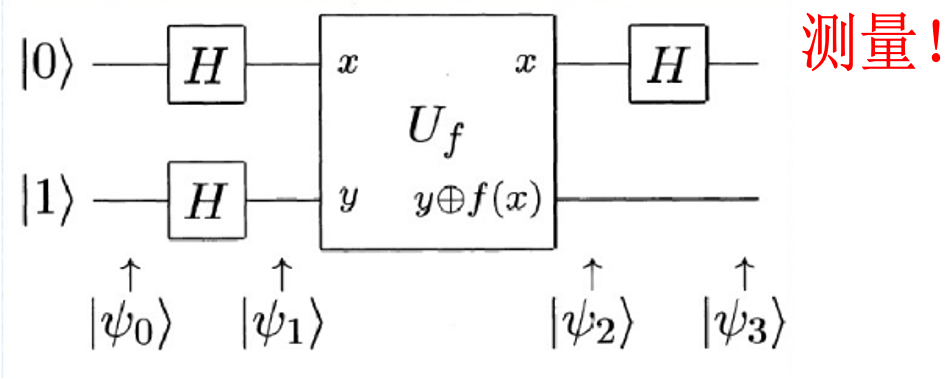
\includegraphics[width=0.5\textwidth]{figs/34.png}
    \end{center}
    算法推导:
    \begin{itemize}
        \item $\rs{\psi_0}=\rs{0}\rs{1}$
        \item $\rs{\psi_1}=H\rs{0}H\rs{1}=\Pstate\Mstate$
    \end{itemize}
\end{frame}

\begin{frame}
    \frametitle{}
     令:$\rs{\psi_1}=\rs{x}\Mstate$ \\
     有:$U_f\rs{\psi_1}=\rs{x}\dfrac{\rs{0\oplus f(x)}-\rs{1\oplus f(x)}}{\sqrt{2}}= \rs{x}(-1)^{f(x)} \Mstate$ \\
     \[\text{if} ~f(x)=0, \quad \frac{\rs{0\oplus f(x)}-\rs{1\oplus f(x)}}{\sqrt{2}}=\frac{\rs{0\oplus 0}-\rs{1\oplus 0}}{\sqrt{2}} = (-1)^{f(x)=0} \Mstate\]
     \[\text{if} ~f(x)=1, \quad \frac{\rs{0\oplus f(x)}-\rs{1\oplus f(x)}}{\sqrt{2}}=\frac{\rs{0\oplus 1}-\rs{1\oplus 1}}{\sqrt{2}} = (-1)^{f(x)=1} \Mstate\]
    \[\rs{\psi_2}= \Pstate \dfrac{\rs{0\oplus f(x)}-\rs{1\oplus f(x)}}{\sqrt{2}}= \dfrac{\rs{0}(-1)^{f(0)}+ \rs{1}(-1)^{f(1)} }{\sqrt{2}} \Mstate\]
\end{frame}

\begin{frame}
    \frametitle{}
     \[\text{if} ~f(0)=f(1), \quad \rs{\psi_2}=\Pstate \Mstate, \quad \rs{\psi_3} =H\rs{\psi_2}=\rs{0}\Mstate \]
     \[\text{if} ~f(0)\neq f(1), \quad\rs{\psi_2}=\Mstate \Mstate,  \quad \rs{\psi_3} =H\rs{\psi_2}=\rs{1}\Mstate \]
    测量第一个位,如果是“0”,$f(x)$是常函数,否则是平衡函数。
\end{frame}

\section{3. Deutsch-Jozsa 算法}
\begin{frame}
    \frametitle{Deutsch-Jozsa 算法}
    {\Bullet}~任务:Alice 从$0$到$(2^n -1)$中选取一个整数$x$送给Bob. Bob应用某个常函数(对所有的x,都有相同的f(x)或者平衡函数(对所有的x,f(x)有一半概率取“0”,另一半概率取“1”)进行计算,并把函数结果$f(x)$发回给Alice.
    Alice 猜 Bob 使用的函数是常函数还是平衡函数。请Alice 猜几次才能成功。 \\ \vspace{0.8em}
    {\Bullet}~经典算法最少两次,最多 $(2^n)/2+1$次
    \begin{itemize}
        \item (1)第一次返回$f(x_1)$,第二次返回$f(x_2)$, 若$f(x_1)\neq f(x_2)$ 平衡函数!
        \item (2)若$f(x_1) = f(x_2)$,并不能说明是常函数,因为平衡函数有一半概率函数值相同,游戏继续!
        \item (3) 最差的情况是,$(2^n)/2$次的结果都相同,则依然不能判定!
        \item (4) $(2^n)/2+1$次的结果与前面的还相同,则说明是常函数,否则是平衡函数。
    \end{itemize}
\end{frame}

\begin{frame}
    \frametitle{}
    {\Bullet}~量子算法只需一次!算法线路如下图
    \begin{center}
        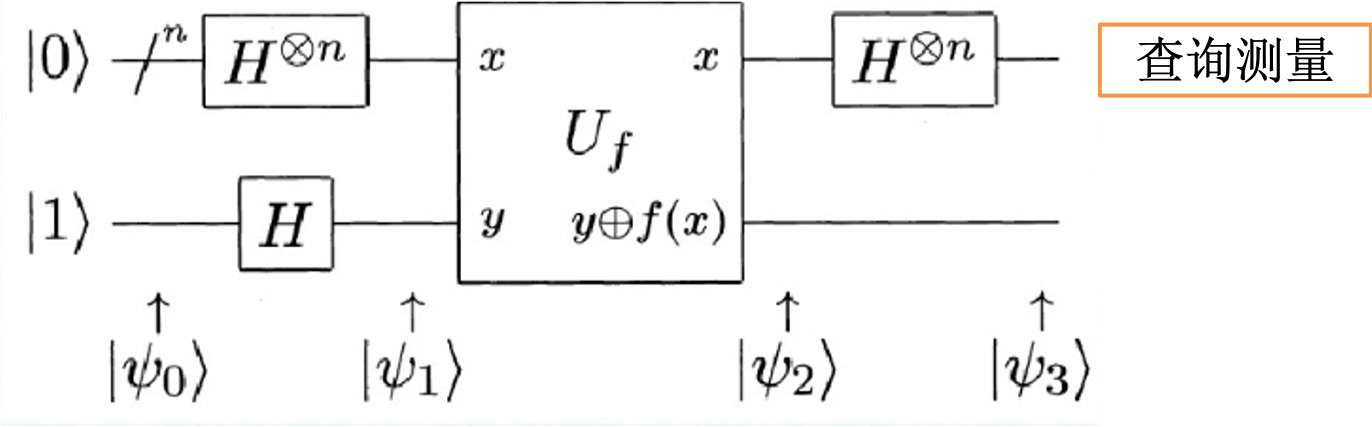
\includegraphics[width=0.66\textwidth]{figs/35.png}
    \end{center}
    {\Bullet}~算法推导:
    \begin{itemize}
        \item $\rs{\psi_0}=\rs{0}\rs{0}\cdots\rs{0}\rs{1}=\rs{0}^{\otimes n}\rs{1}$
        \item $\rs{\psi_1}=H^{\otimes n}\rs{0}^{\otimes n}H\rs{1}=[\Pstate]^{\otimes n} \Mstate = \sum\limits_x \dfrac{\rs{x}}{\sqrt{2^n}} \Mstate $
    \end{itemize}
    求和是对所有的计算基矢态 ($2^n$个,即$\rs{00\cdots 0},\rs{00\cdots 1},\rs{11\cdots 1}$)
\end{frame}

\begin{frame}
    \frametitle{}
     $\rs{\psi_1}=\sum\limits_x \dfrac{\rs{x}}{\sqrt{2^n}} \Mstate$ \\
     $U_f\rs{\psi_1}=\sum\limits_x \dfrac{\rs{x}}{\sqrt{2^n}} [\dfrac{\rs{0\oplus f(x)}}{\sqrt{2}}]- \sum\limits_x \dfrac{\rs{x}}{\sqrt{2^n}}[\dfrac{\rs{1\oplus f(x)}}{\sqrt{2}}]$ \\
     $\hspace{3em}= \sum\limits_x \dfrac{\rs{x}}{\sqrt{2^n}}[\dfrac{\rs{0\oplus f(x)}}{\sqrt{2}}-\dfrac{\rs{1\oplus f(x)}}{\sqrt{2}}]$ \\
     \[\text{if} ~f(x)=0, \quad \frac{\rs{0\oplus f(x)}-\rs{1\oplus f(x)}}{\sqrt{2}}=\frac{\rs{0\oplus 0}-\rs{1\oplus 0}}{\sqrt{2}} = (-1)^{f(x)=0} \Mstate\]
     \[\text{if} ~f(x)=1, \quad \frac{\rs{0\oplus f(x)}-\rs{1\oplus f(x)}}{\sqrt{2}}=\frac{\rs{0\oplus 1}-\rs{1\oplus 1}}{\sqrt{2}} = (-1)^{f(x)=1} \Mstate\]
    $\rs{\psi_2}= \sum\limits_x \dfrac{(-1)^{f(x)}\rs{x}}{\sqrt{2^n}} \Mstate$
\end{frame}

\begin{frame}
    \frametitle{}
    \[\begin{aligned}
        \rs{\psi_3} &= H^{\otimes n }\rs{\psi_2}\\
        &= H^{\otimes n } \sum\limits_x \dfrac{(-1)^{f(x)}\rs{x}}{\sqrt{2^n}} \Mstate\\ 
        &=  \sum\limits_x \dfrac{(-1)^{f(x)}H^{\otimes n }\rs{x}}{\sqrt{2^n}} \Mstate\\ 
        &=  \sum\limits_x \dfrac{(-1)^{f(x)}}{\sqrt{2^n}} \sum\limits_z \dfrac{(-1)^{x\cdot z}\rs{z}}{\sqrt{2^n}} \Mstate\\   
        &=  \sum\limits_{x,z} \dfrac{(-1)^{x\cdot z+f(x)}\rs{z}}{2^n} \Mstate 
    \end{aligned}\]
\end{frame}

\begin{frame}
    \frametitle{}
    \[
    \rs{\psi_3}=\sum\limits_{x,z} \dfrac{(-1)^{x\cdot z+f(x)}}{2^n}\rs{z} \Mstate 
    \]
    考察上式中的第一项$\rs{z}=\rs{00\cdots 0}$项\\
    \[\sum\limits_{x,z} \dfrac{(-1)^{x\cdot z+f(x)}}{2^n}\rs{z}=\sum\limits_{x} \dfrac{(-1)^{f(x)}}{2^n}\rs{00\cdots0}\]
    分析:当f(x)为常函数时,f(x)都一样(0 或1), 这一项的振幅必然为1或-1,由于$\psi_3$是归一化的,模长是1,意味着除第一项外的所有其他项的振幅都为“0”.因此当Alice测一次,如果得的都是“$\rs{00\cdots0}$”,则Bob用的是常函数,否则为平衡函数。
\end{frame}

\begin{frame}
    \frametitle{附录}
    (1)单位操作
    \[H \rs{0}=\frac{\rs{0}+\rs{1}}{\sqrt{2}}\]
    \[H \rs{1}=\frac{\rs{0}-\rs{1}}{\sqrt{2}}\]
    {\Bullet} 统一表示为:(x,z 分别取0或1)\\
    \[H \rs{x}=\frac{\sum_z(-1)^{xz}\rs{z}}{\sqrt{2}}\]
\end{frame}

\begin{frame}
    \frametitle{}
    (2)双位操作
    \[H^{\otimes 2} \rs{00}=\Pstate\Pstate=\frac{\rs{00}}{\sqrt{2^2}}+\frac{\rs{01}}{\sqrt{2^2}}+ \frac{\rs{10}}{\sqrt{2^2}}+ \frac{\rs{11}}{\sqrt{2^2}}\]
    \[H^{\otimes 2} \rs{01}=\Pstate\Mstate=\frac{\rs{00}}{\sqrt{2^2}}-\frac{\rs{01}}{\sqrt{2^2}}+ \frac{\rs{10}}{\sqrt{2^2}}- \frac{\rs{11}}{\sqrt{2^2}}\]
    \[H^{\otimes 2} \rs{10}=\Mstate\Pstate=\frac{\rs{00}}{\sqrt{2^2}}+\frac{\rs{01}}{\sqrt{2^2}}- \frac{\rs{10}}{\sqrt{2^2}}- \frac{\rs{11}}{\sqrt{2^2}}\]
    \[H^{\otimes 2} \rs{11}=\Mstate\Mstate=\frac{\rs{00}}{\sqrt{2^2}}-\frac{\rs{01}}{\sqrt{2^2}}- \frac{\rs{10}}{\sqrt{2^2}}+ \frac{\rs{11}}{\sqrt{2^2}}\]
    {\Bullet} 统一表示为:($x_1,x_2,z_1,z_2$ 分别取0或1)\\
    \[H^{\otimes 2} \rs{x_1x_2}=\frac{\sum_{z_1z_2}(-1)^{x_1z_1+x_2z_2}\rs{z_1z_2}}{\sqrt{2^2}}\]
\end{frame}

\begin{frame}
    \frametitle{}
    \[H^{\otimes 2} \rs{x}=\frac{\sum_{z}(-1)^{x\cdot z}\rs{z}}{\sqrt{2^2}}\]
    (3)推广到n位操作
    \[H^{\otimes n} \rs{x}=\frac{\sum_{z}(-1)^{x\cdot z}\rs{z}}{\sqrt{2^n}}\]
\end{frame}